\section{Final Thoughts}
% Guinard le llama "Final Thoughts" => me mola más
% Almeida le llama "Final Remarks"


% camino dificil en el que ha habido mucho estudio de otras soluciones, pero también de experimentación practica: probando y descartando conceptos para gradualmente mejorar el middleware
% echar vista atras en todo lo hecho desde Jxta hasta hoy!
This dissertation is the result of years of work towards a \acl{tsc} middleware for \acl{ubicomp}.
It describes the latest shape of the idea which I began sketching even before I finally decided to start this thesis.
% en esa mejora contribuyeron: proyectos, colegas cientificos de Deusto y otras muchas universidades en reuniones informales, estancia o conferencias
But the evolution of this idea would not have been possible without other researchers who have directly or indirectly help me. % direct: feedback de alguna forma; indirect: publicaciones que he podido leer
%idea which has evolve thanks to the research community. 
% Cura de humildad diciendo lo que querrias haber conseguido
In the same way, I hope that this thesis will contribute or inspire at some degree to the scientific community.

\bigskip

% http://en.wikipedia.org/wiki/Standing_on_the_shoulders_of_giants
% Adaptado de:
%    http://www.flickr.com/photos/mushon/282287572/
%    http://www.flickr.com/photos/futurefashion/130994094/sizes/z/
\begin{figure}[h]
    \centering
    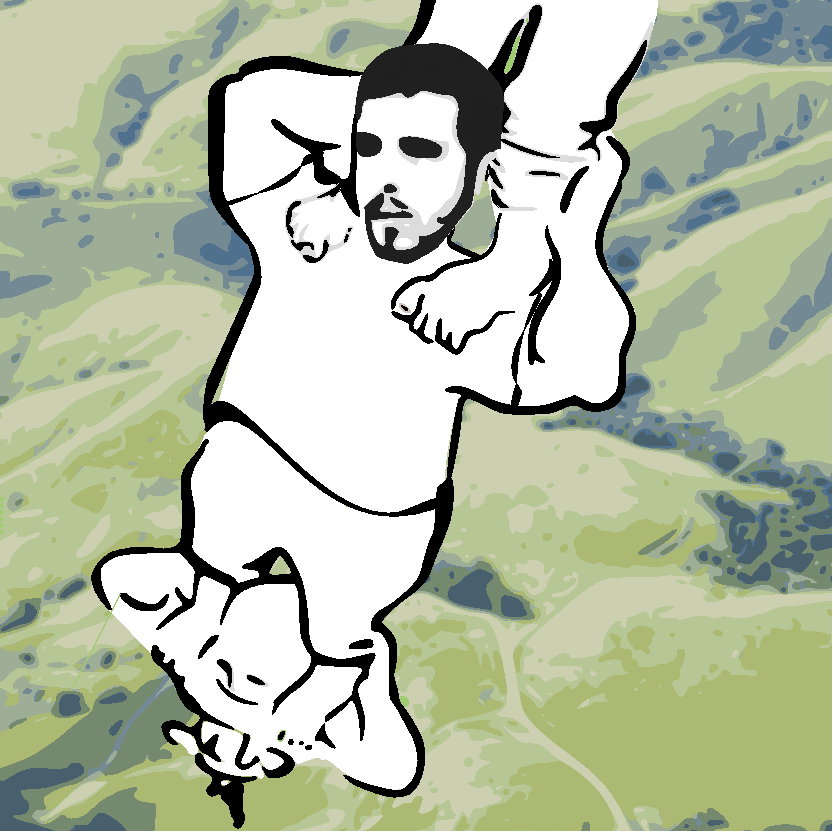
\includegraphics[width=0.7\textwidth]{shoulders}
    \caption*{}{\quote{If I have seen further it is by standing on the shoulders of giants.} \qauthor{Isaac Newton}}
    \label{fig:shouldersOfGiants}
\end{figure}